
\section{La Abstracción de las RNN}

Si bien las representaciones derivadas de las redes convolucionales ofrecen cierta sensibilidad al orden de las palabras, su sensibilidad al orden se limita principalmente a patrones locales y no tiene en cuenta el orden de patrones que están lejos en la secuencia. Las redes neuronales recurrentes (RNN) permiten representar entradas secuenciales de longitud arbitraria en vectores de tamaño fijo, prestando atención a las propiedades estructuradas de las entradas \cite{goldberg2016primer}. Las RNN, especialmente aquellas con arquitecturas con compuertas como LSTM y GRU, son muy eficaces para capturar regularidades estadísticas en entradas secuenciales.

Utilizamos $\vec{x}_{i:j}$ para denotar la secuencia de vectores $\vec{x}_i, \dots, \vec{x}_j$. A alto nivel, la RNN es una función que toma como entrada una secuencia ordenada de longitud arbitraria de $n$ vectores de dimensión $d_{in}$, $\vec{x}_{1 :n}=\vec{x}_1,\vec{x}_2, \dots, \vec{x}_n$ ($\vec{x}_i \in \mathbb{R}^{d_{in}}$), y devuelve como salida un solo vector de dimensión $d_{out}$, $\vec{y}_n \in \mathbb{R}^{d_{out}}$:

\begin{equation}
\begin{split}
\vec{y}_n & = \text{RNN}(\vec{x}_{1:n}) \\
\vec{x}_i \in \mathbb{R}^{d_{in}}, & \quad \vec{y}_n \in \mathbb{R}^{d_{out}}
\end{split}
\end{equation}

Esto define implícitamente un vector de salida $\vec{y}_i$ para cada prefijo $\vec{x}_{1:i}$ de la secuencia $\vec{x}_{i:n}$. Denotamos por $RNN^{*}$ a la función que devuelve esta secuencia:

\begin{equation}
\begin{split}
\vec{y}_{1:n} & = RNN^{*}(\vec{x}_{1:n}) \\
\vec{y}_i & = \text{RNN}(\vec{x}_{1:i}) \\
\vec{x}_i \in \mathbb{R}^{d_{in}}, & \quad \vec{y}_n \in \mathbb{R}^{d_{out}}
\end{split}
\end{equation}

Luego, se utiliza el vector de salida $\vec{y}_n$ para realizar predicciones adicionales. Por ejemplo, un modelo para predecir la probabilidad condicional de un evento $e$ dado la secuencia $\vec{x}_{1:n}$ se puede definir como el $j$-ésimo elemento del vector de salida resultante de la operación softmax sobre una transformación lineal de la codificación RNN:

\begin{displaymath}
p(e = j|\vec{x}_{1:n}) = \text{softmax}(\text{RNN}(\vec{x}_{1:n})\cdot W +\vec{b})_{[j]}
\end{displaymath}

La función RNN proporciona un marco para condicionar toda la historia sin recurrir a la suposición de Markov que se utiliza tradicionalmente para modelar secuencias. La RNN se define de forma recursiva mediante una función $R$ que toma como entrada un vector de estado $\vec{s}_{i-1}$ y un vector de entrada $\vec{x}_{i}$, y devuelve un nuevo vector de estado $\vec{s}_i$. Luego, el vector de estado $\vec{s}_i$ se asigna a un vector de salida $\vec{y}_i$ mediante una función determinista simple $O(\cdot)$. La base de la recursión es un vector de estado inicial $\vec{s}_{0}$, que también es una entrada de la RNN. Por brevedad, a menudo omitimos el vector inicial $\vec{s}_{0}$ o asumimos que es el vector cero. Al construir una RNN, al igual que al construir una red de alimentación directa, es necesario especificar la dimensión de las entradas $\vec{x}_i$, así como las dimensiones de las salidas $\vec{y}_i$:

\begin{equation}
\begin{split}
RNN^{*}(\vec{x}_{1:n};\vec{s}_0) & = \vec{y}_{1:n} \\
\vec{y}_i & = O(\vec{s}_i) \\
\vec{s}_i & = R(\vec{s}_{i-1},\vec{x}_i) \\
\vec{x}_i \in \mathbb{R}^{d_{in}}, & \quad \vec{y}_i \in \mathbb{R}^{d_{out}}, \quad \vec{s}_i \in \mathbb{R}^{f(d_{out})}
\end{split}
\end{equation}

Las funciones $R$ y $O$ son las mismas en todas las posiciones de la secuencia. La RNN realiza un seguimiento de los estados de la computación a través del vector de estado $\vec{s}_i$ que se guarda y se pasa en las invocaciones de $R$.

\begin{figure}[h]
  \centering
  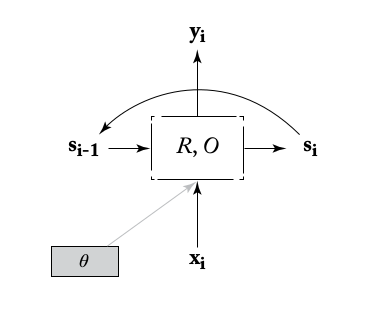
\includegraphics[scale=0.4]{pics/RNN.png}
  \caption{Representación gráfica de una RNN.}
\end{figure}

Esta presentación sigue la definición recursiva y es válida para secuencias de longitud arbitraria. Sin embargo, para una secuencia de entrada de tamaño finito (y todas las secuencias de entrada con las que trabajamos son finitas), se puede desenrollar la recursión.

\begin{figure}[h]
  \centering
  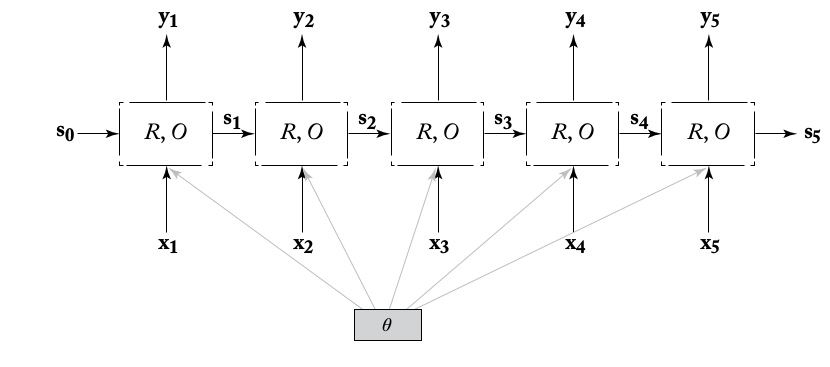
\includegraphics[scale=0.35]{pics/RNN-unrolled.png}
  \caption{Representación gráfica de una RNN desenrollada para una secuencia de longitud finita.}
\end{figure}

Los parámetros $\theta$ resaltan el hecho de que los mismos parámetros se comparten en todos los pasos de tiempo. Diferentes instancias de $R$ y $O$ darán como resultado estructuras de red diferentes. Observamos que el valor de $\vec{s}_i$ (y, por lo tanto, $\vec{y}_i$) se basa en toda la entrada $\vec{x}_1,\dots, \vec{x}_i$. Por ejemplo, al expandir la recursión para $i = 4$ obtenemos:

\begin{figure}[h]
  \centering
  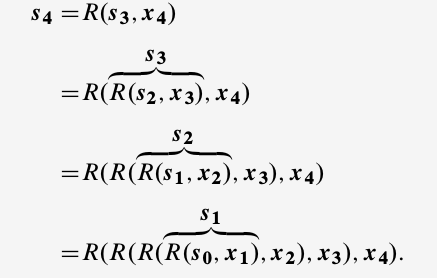
\includegraphics[scale=0.35]{pics/RNN-recursion.png}
  \caption{Representación gráfica de la RNN después de expandir la recursión.}
\end{figure}

Así, $\vec{s}_n$ y $\vec{y}_n$ pueden considerarse como la codificación de toda la secuencia de entrada. El objetivo del entrenamiento de la red es establecer los parámetros de $R$ y $O$ de manera que el estado transmita información útil para la tarea que estamos tratando de resolver.

\section{Red Elman o Simple-RNN}

Después de describir la abstracción de las RNN, ahora podemos discutir las instancias más simples de estas. Recordemos que estamos interesados en una función recursiva $\vec{s}_i = R(\vec{x}_i, \vec{s}_{i-1})$ tal que $\vec{s}_i$ codifique la secuencia $\vec{x}_{1:n}$. La formulación más sencilla de una RNN se conoce como Red Elman o Simple-RNN (S-RNN).

\begin{equation}
\begin{split}
\vec{s}_i & = R_{SRNN}(\vec{x}_{i},\vec{s}_{i-1}) = g(\vec{s}_{i-1}W^{s}+\vec{x}_{i}W^{x}+\vec{b}) \\
\vec{y}_i & = O_{SRNN}(\vec{s}_i) = \vec{s}_i \\
\vec{s}_i, \vec{y}_i \in \mathbb{R}^{d_{s}}, & \quad \vec{x}_i \in \mathbb{R}^{d_{x}}, \quad W^{x} \in \mathbb{R}^{d_{x}\times d_{s}}, \quad W^{s} \in \mathbb{R}^{d_{s}\times d_{s}}, \vec{b} \in \mathbb{R}^{d_{s}}
\end{split}
\end{equation}

El estado $\vec{s}_i$ y la entrada $\vec{x}_i$ se transforman linealmente. Los resultados se suman (junto con un término de sesgo) y luego se pasan a través de una función de activación no lineal $g$ (comúnmente tangente hiperbólica o ReLU). El Simple-RNN ofrece buenos resultados para etiquetado de secuencias y modelado del lenguaje.

\begin{figure}[h]
  \centering
  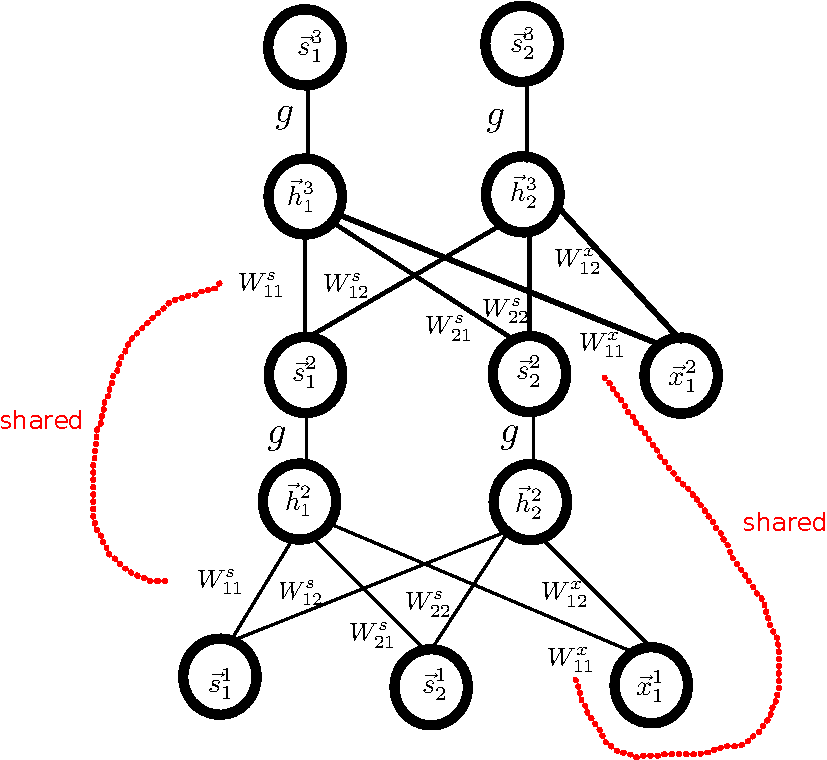
\includegraphics[scale=0.55]{pics/elman.pdf}
  \caption{Red Elman o Simple-RNN.}
\end{figure}

\section{Entrenamiento de las RNN}

Una RNN desenrollada es simplemente una red neuronal muy profunda. Los mismos parámetros se comparten en muchas partes de la computación y se agrega una entrada adicional en varias capas. Para entrenar una red RNN, se necesita crear el grafo computacional desenrollado para una secuencia de entrada dada, agregar un nodo de pérdida al grafo desenrollado y luego utilizar el algoritmo de retropropagación para calcular los gradientes con respecto a esa pérdida. Este procedimiento se conoce en la literatura de las RNN como retropropagación a través del tiempo (BPTT). La RNN por sí sola no hace mucho, sino que sirve como un componente entrenable en una red más grande. La predicción final y el cálculo de pérdida se realizan en esa red más grande y el error se retropropaga a través de la RNN. De esta manera, la RNN aprende a codificar propiedades de las secuencias de entrada que son útiles para la tarea de predicción. La señal de supervisión no se aplica directamente a la RNN, sino a través de la red más grande.

\section{Patrones de uso de las RNN: Aceptador}

Un patrón común de uso de las RNN es el patrón del aceptador. Este patrón se utiliza para la clasificación de texto, donde la señal de supervisión se basa únicamente en el vector de salida final $\vec{y}_n$. El vector de salida de la RNN $\vec{y}_n$ se alimenta a una capa completamente conectada o un MLP, que produce una predicción. Los gradientes de error luego se retropropagan a través del resto de la secuencia. La pérdida puede tener cualquier forma conocida, como entropía cruzada o hinge, etc.

\begin{figure}[h]
  \centering
  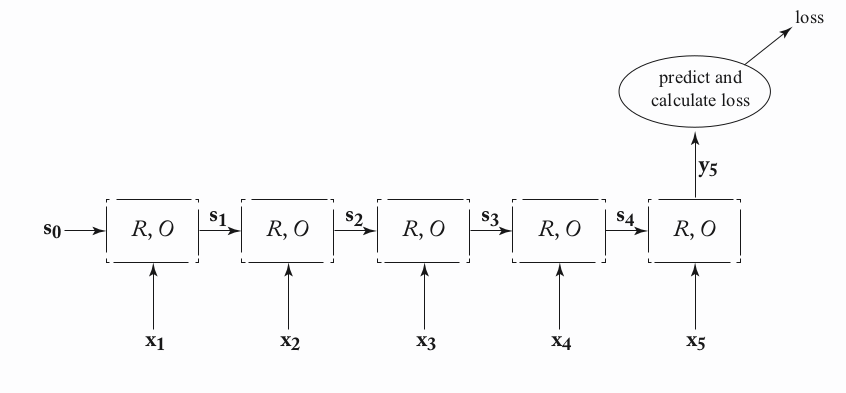
\includegraphics[scale=0.3]{pics/acceptor.png}
  \caption{Gráfico de entrenamiento de una RNN del tipo aceptador.}
\end{figure}

Por ejemplo, se puede tener una RNN que lee los caracteres de una palabra uno por uno y luego utiliza el estado final para predecir la categoría gramatical de esa palabra. Otro ejemplo es una RNN que lee una oración y, en función del estado final, decide si transmite un sentimiento positivo o negativo.

\section{Patrones de uso de las RNN: Transductor}

Otra opción es tratar la RNN como un transductor, produciendo una salida $\hat{t}_i$ para cada entrada que lee. Este patrón es muy útil para tareas de etiquetado de secuencias (por ejemplo, etiquetado de partes del discurso, reconocimiento de entidades nombradas, etc.). Se calcula una señal de pérdida local (por ejemplo, entropía cruzada) $L_{\text{local}}(\hat{t}_{i},{t}_{i})$ para cada una de las salidas $\hat{t}_{i}$ basada en una etiqueta verdadera ${t}_{i}$. La pérdida para la secuencia desenrollada será entonces: $L(\hat{t}_{i:n},{t}_{i:n}) = \sum_{i}L_{\text{{local}}}(\hat{t}_{i},{t}_{i})$, o utilizando otra combinación en lugar de la suma, como el promedio o un promedio ponderado.

\begin{figure}[h]
  \centering
  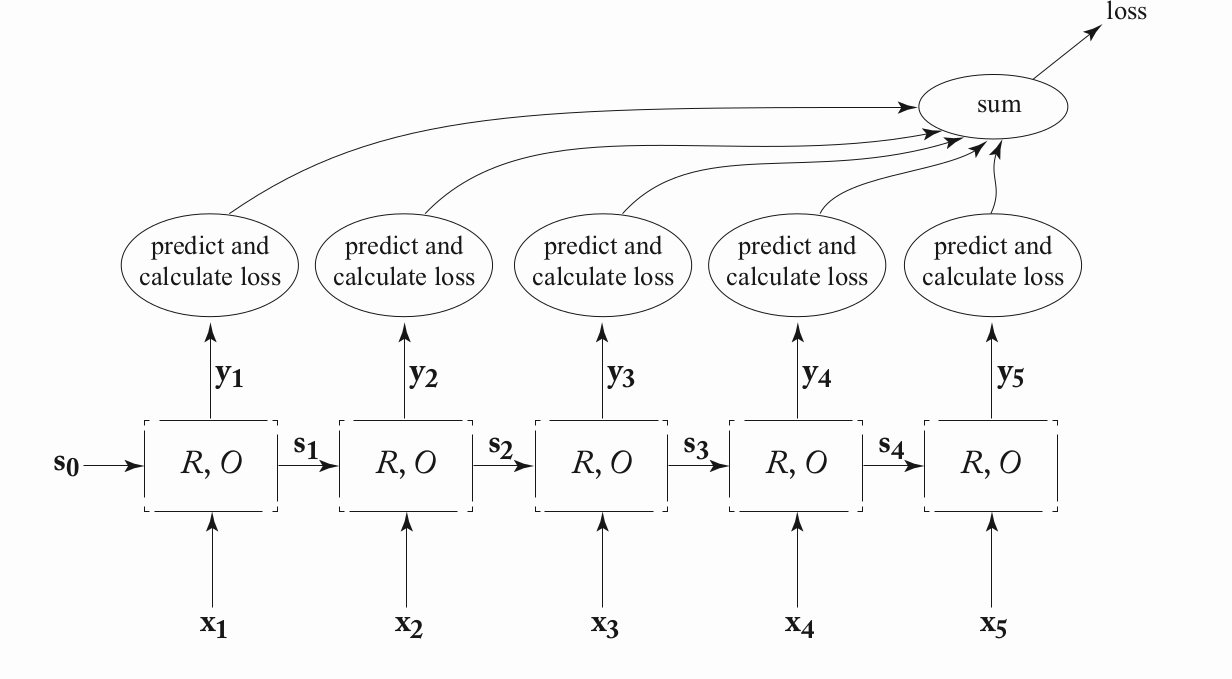
\includegraphics[scale=0.25]{pics/transducer.png}
  \caption{Gráfico de entrenamiento de una RNN del tipo transductor.}
\end{figure}

Por ejemplo, un etiquetador de secuencias (por ejemplo, NER, POS), en el que $\vec{x}_{i:n}$ representa las representaciones de características de las $n$ palabras de una oración, y $t_i$ se utiliza para predecir la asignación de etiquetas de la palabra $i$ en función de las palabras $1:i$. Otro ejemplo es el modelado de lenguaje, en el que la secuencia de palabras $x_{1:n}$ se utiliza para predecir una distribución sobre la palabra $(i+1)$-ésima. Los modelos de lenguaje basados en RNN han demostrado tener una perplejidad mucho mejor que los modelos de lenguaje tradicionales.

El uso de las RNN como transductores nos permite relajar la suposición de Markov que se hace tradicionalmente en los modelos de lenguaje y los etiquetadores HMM, y condicionar en todo el historial de predicciones.

\section{Redes neuronales recurrentes bidireccionales (BIRNN)}

Una elaboración útil de una RNN es una red neuronal recurrente bidireccional (también conocida como biRNN). Consideremos la tarea de etiquetado de secuencias en una oración. Una RNN nos permite calcular una función de la $i$-ésima palabra $x_i$ en función de las palabras anteriores $x_{1:i}$, incluyendo la palabra actual. Sin embargo, las palabras siguientes $x_{i+1:n}$ también pueden ser útiles para la predicción. La biRNN nos permite mirar arbitrariamente lejos tanto al pasado como al futuro dentro de la secuencia. Consideremos una secuencia de entrada $\vec{x}_{1:n}$. La biRNN funciona manteniendo dos estados separados, $s_{i}^{f}$ y $s_{i}^{b}$ para cada posición de entrada $i$. El estado hacia adelante $s_{i}^{f}$ se basa en $\vec{x}_1, \vec{x}_2, \dots ,\vec{x}_i$, mientras que el estado hacia atrás $s_{i}^{b}$ se basa en $\vec{x}_n, \vec{x}_{n-1}, \dots ,\vec{x}_i$. Los estados hacia adelante y hacia atrás se generan mediante dos RNN diferentes. La primera RNN $(R^f, O^f)$ recibe la secuencia de entrada $\vec{x}_{1:n}$ tal como está, mientras que la segunda RNN $(R^b , O^b)$ recibe la secuencia de entrada en orden inverso. La representación del estado $\vec{s}_i$ está compuesta tanto por los estados hacia adelante como por los estados hacia atrás. La salida en la posición $i$ se basa en la concatenación de los dos vectores de salida:

\begin{displaymath}
\vec{y}_i = [\vec{y}_{i}^{f};\vec{y}_{i}^{b}]=[O^{f}(s_{i}^{f});O^{b}(s_{i}^{b})]
\end{displaymath}

La salida tiene en cuenta tanto el pasado como el futuro. La codificación biRNN de la palabra $i$ en una secuencia es la concatenación de dos RNN, una que lee la secuencia desde el principio y otra que la lee desde el final. Definimos $biRNN(\vec{x}_{1:n}, i)$ como el vector de salida correspondiente a la $i$-ésima posición de la secuencia:

\begin{displaymath}
biRNN(\vec{x}_{1:n}, i) = \vec{y}_i = [RNN^{f}(\vec{x}_{1:i});RNN^{b}(\vec{x}_{n:i})]
\end{displaymath}

El vector $\vec{y}_i$ se puede utilizar directamente para la predicción o se puede alimentar como parte de la entrada a una red más compleja. Mientras que las dos RNN se ejecutan de forma independiente, los gradientes de error en la posición $i$ fluirán tanto hacia adelante como hacia atrás a través de las dos RNN. Al alimentar el vector $\vec{y}_i$ a través de un MLP antes de la predicción, se mezclarán aún más las señales hacia adelante y hacia atrás.

\begin{figure}[h]
  \centering
  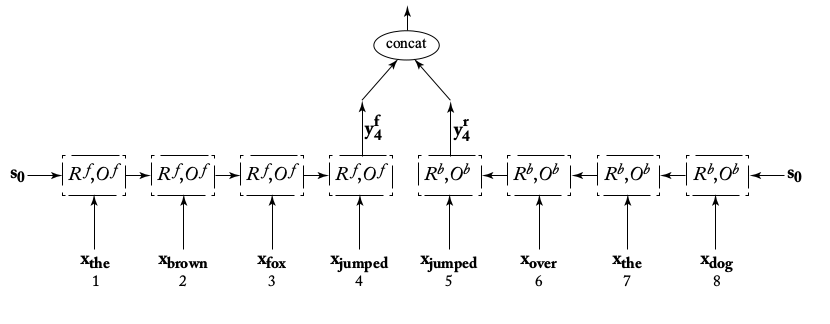
\includegraphics[scale=0.35]{pics/biRNN.png}
  \caption{Red neuronal recurrente bidireccional (biRNN).}
\end{figure}

Observa cómo el vector $\vec{y}_4$, correspondiente a la palabra \textbf{saltó}, codifica una ventana infinita alrededor (e incluyendo) el vector de enfoque $\vec{x}_{\text{saltó}}$. La biRNN es muy efectiva para tareas de etiquetado, en las que cada vector de entrada corresponde a un vector de salida. También es útil como componente de extracción de características entrenable de propósito general, que se puede utilizar siempre que se requiera una ventana alrededor de una palabra determinada.

\section{Redes neuronales recurrentes multi-capa (apiladas)}

Las RNN se pueden apilar en capas, formando una estructura en forma de cuadrícula. Consideremos $k$ RNN, $RNN_{1},\dots, RNN_{k}$, donde la $j$-ésima RNN tiene estados $\vec{s}_{1:n}^{j}$ y salidas $\vec{y}_{1:n}^{j}$. La entrada para la primera RNN son $\vec{x}_{1:n}$. La entrada de la $j$-ésima RNN ($j\geq 2$) son las salidas de la RNN debajo de ella, $\vec{y}_{1:n}^{j-1}$. La salida de toda la formación es la salida de la última RNN, $\vec{y}_{1:n}^k$. Estas arquitecturas en capas se conocen comúnmente como RNN profundas. No

existe una restricción en la cantidad de capas que se pueden apilar, pero es importante tener en cuenta que agregar más capas puede aumentar la complejidad del modelo y requerir más datos y tiempo de entrenamiento.

\begin{figure}[h]
  \centering
  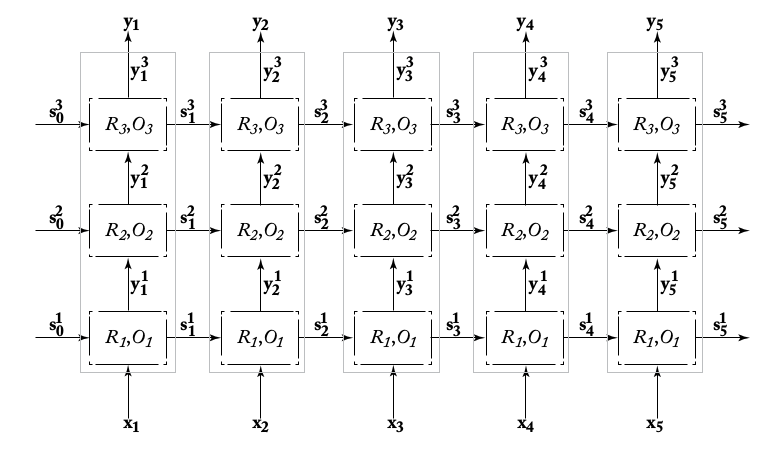
\includegraphics[scale=0.4]{pics/stackedRNN.png}
  \caption{Redes neuronales recurrentes multi-capa (apiladas).}
\end{figure}

La ventaja de las RNN apiladas es que cada capa puede aprender representaciones de características de nivel superior en la secuencia de entrada. Las capas superiores pueden capturar patrones de más largo alcance y dependencias más complejas. Cada capa procesa la secuencia de entrada de manera incremental, y las capas superiores reciben información de las capas inferiores para ayudar a hacer predicciones más precisas. Las RNN apiladas son particularmente efectivas para tareas de modelado del lenguaje y traducción automática.


\section{Arquitecturas con compuertas}
Hasta ahora hemos visto solo una instancia de la RNN: la RNN simple (S-RNN) o red Elman. Este modelo es difícil de entrenar efectivamente debido al problema de los \textbf{gradientes que desaparecen}. Las señales de error (gradientes) en pasos posteriores de la secuencia disminuyen rápidamente en el proceso de retropropagación, por lo que no llegan a las señales de entrada anteriores, lo que dificulta que la S-RNN capture dependencias a largo plazo. Las arquitecturas basadas en compuertas, como LSTM \cite{hochreiter1997long} y GRU \cite{cho2014learning}, están diseñadas para solucionar esta deficiencia.

Intuitivamente, las redes neuronales recurrentes pueden considerarse como redes de alimentación profunda con parámetros compartidos entre diferentes capas. En el caso de la RNN simple, los gradientes incluyen multiplicaciones repetidas de la matriz $W$, lo que hace muy probable que los valores desaparezcan o exploten. El mecanismo de las compuertas mitiga este problema en gran medida al eliminar esta multiplicación repetida de una sola matriz.

Podemos considerar la RNN como un dispositivo de computación de propósito general, donde el estado $\vec{s}_i$ representa una memoria finita. Cada aplicación de la función $R$ lee una entrada $\vec{x}_{i+1}$, lee la memoria actual $\vec{s}_i$, opera en ellas de alguna manera y escribe el resultado en la memoria. Esto resulta en un nuevo estado de memoria $\vec{s}_{i+1}$. Sin embargo, un problema aparente con la arquitectura S-RNN es que el acceso a la memoria no está controlado. En cada paso de la computación, se lee todo el estado de memoria y se escribe todo el estado de memoria. ¿Cómo se puede proporcionar un acceso a la memoria más controlado?

Podemos utilizar un vector binario $\vec{g} \in [0,1]^n$ que actúa como una \textbf{compuerta} para controlar el acceso a vectores de dimensión $n$ utilizando la operación producto de Hadamard $\vec{x} \odot \vec{g}$. La operación Hadamard es la multiplicación elemento a elemento de dos vectores:
\begin{displaymath}
\vec{x} = \vec{u} \odot \vec{v}  \Leftrightarrow  \vec{x}_{[i]} = \vec{u}_{[i]} \cdot \vec{v}_{[i]} \quad \forall i \in [1,n]
\end{displaymath}

Si consideramos una memoria $\vec{s} \in \mathbb{R}^{d}$, una entrada $\vec{x} \in \mathbb{R}^{d}$ y una compuerta $\vec{g} \in [0,1]^{d}$, la siguiente computación:
\begin{displaymath}
\vec{s}' \leftarrow \vec{g} \odot \vec{x} + (\vec{1}-\vec{g}) \odot (\vec{s})
\end{displaymath}
lee las entradas en $\vec{x}$ que corresponden a los valores $\vec{1}$ en $\vec{g}$ y las escribe en la nueva memoria $\vec{s}'$. Las ubicaciones que no se leyeron se copian de la memoria $\vec{s}$ a la nueva memoria $\vec{s}'$ mediante el uso de la compuerta $(\vec{1}-\vec{g})$.

Este mecanismo de compuerta puede servir como un bloque de construcción en nuestra RNN. Los vectores de compuerta se pueden utilizar para controlar el acceso al estado de memoria $\vec{s}_i$. Sin embargo, todavía nos faltan dos componentes importantes (y relacionados): 1) las compuertas no deben ser estáticas, sino que deben estar controladas por el estado de memoria actual y la entrada, y 2) su comportamiento debe ser aprendido.

Esto presenta un obstáculo, ya que el aprendizaje en nuestro marco implica ser diferenciable (debido al algoritmo de retropropagación). Los valores binarios de 0-1 utilizados en las compuertas no son diferenciables. Una solución a este problema es aproximar el mecanismo de compuerta dura con un mecanismo de compuerta suave, pero diferenciable.

Para lograr compuertas diferenciables, reemplazamos el requisito de que $\vec{g} \in [0,1]^n$ y permitimos números reales arbitrarios $\vec{g}' \in \mathbb{R}^n$. Estos números reales luego pasan a través de una función sigmoide $\sigma(\vec{g}')$, lo que limita los valores en el rango $(0,1)$, con la mayoría de los valores cerca de los bordes. Al utilizar la compuerta $\sigma(\vec{g}')\odot \vec{x}$, los índices en $\vec{x}$ que corresponden a valores cercanos a uno en $\sigma(\vec{g}')$ pueden pasar, mientras que los que corresponden a valores cercanos a cero son bloqueados. Los valores de las compuertas pueden condicionarse a la entrada y al estado de memoria actual, y pueden entrenarse utilizando un método basado en gradientes para realizar un comportamiento deseado.

Este mecanismo de compuerta controlable es la base de las arquitecturas LSTM y GRU. En cada paso de tiempo, los mecanismos de compuerta diferenciables deciden qué partes de las entradas se escribirán en la memoria y qué partes de la memoria se sobrescribirán (olvidarán).

\section{LSTM}
La arquitectura LSTM (Long Short-Term Memory) \cite{hochreiter1997long} fue diseñada para resolver el problema de los gradientes que desaparecen. Fue la primera arquitectura en introducir el mecanismo de compuertas. La arquitectura LSTM divide explícitamente el vector de estado $\vec{s}_i$ en dos mitades: 1) celdas de memoria y 2) memoria de trabajo. Las celdas de memoria están diseñadas para preservar la memoria, así como los gradientes de error, a lo largo del tiempo, y están controladas mediante componentes de compuertas diferenciables. En cada estado de entrada, se utiliza una compuerta para decidir cuánta de la nueva entrada debe escribirse en la celda de memoria y cuánto del contenido actual de la celda de memoria debe olvidarse. Matemáticamente, la arquitectura LSTM se define como:

\begin{figure}[h]
\centering
  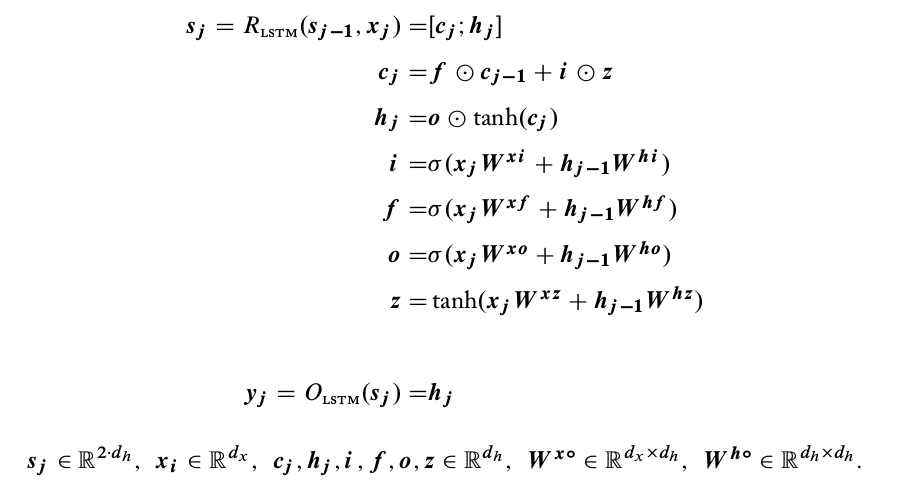
\includegraphics[scale=0.35]{pics/LSTMform.png}
  \caption{Formulación matemática de la arquitectura LSTM.}
\end{figure}

El estado en el tiempo $j$ se compone de dos vectores, $\vec{c}_j$ y $\vec{h}_{j}$, donde $\vec{c}_j$ es el componente de memoria y $\vec{h}_j$ es el componente de estado oculto. Hay tres compuertas, $\vec{i}$, $\vec{f}$ y $\vec{o}$, que controlan la \textbf{entrada} (\textbf{i}nput), \textbf{olvido} (\textbf{f}orget) y \textbf{salida} (\textbf{o}utput), respectivamente. Los valores de las compuertas se calculan en función de las combinaciones lineales de la entrada actual $\vec{x}_j$ y el estado anterior $\vec{h}_{j-1}$, pasados a través de una función de activación sigmoide. Se calcula un candidato de actualización $\vec{z}$ como una combinación lineal de $\vec{x}_j$ y $\vec{h}_{j-1}$, pasados a través de una función de activación tangente hiperbólica (tanh) (para llevar los valores al rango de -1 a 1). Luego, se actualiza la memoria $\vec{c}_j$: la compuerta de olvido controla cuánta de la memoria anterior se debe mantener ($\vec{f} \odot \vec{c}_{j-1}$), y la compuerta de entrada controla cuánta de la actualización propuesta se debe mantener ($\vec{i} \odot  \vec{z}$). Finalmente, el valor de $\vec{h}_j$ (que también es la salida $\vec{y}_j$) se determina en función del contenido de la memoria $\vec{c}_j$, pasado a través de una no linealidad tangente hiperbólica y controlada por la compuerta de salida. Los mecanismos de compuertas permiten que los gradientes relacionados con la parte de memoria $\vec{c}_j$ se mantengan altos en rangos de tiempo muy largos.

\begin{figure}[h]
  \centering
  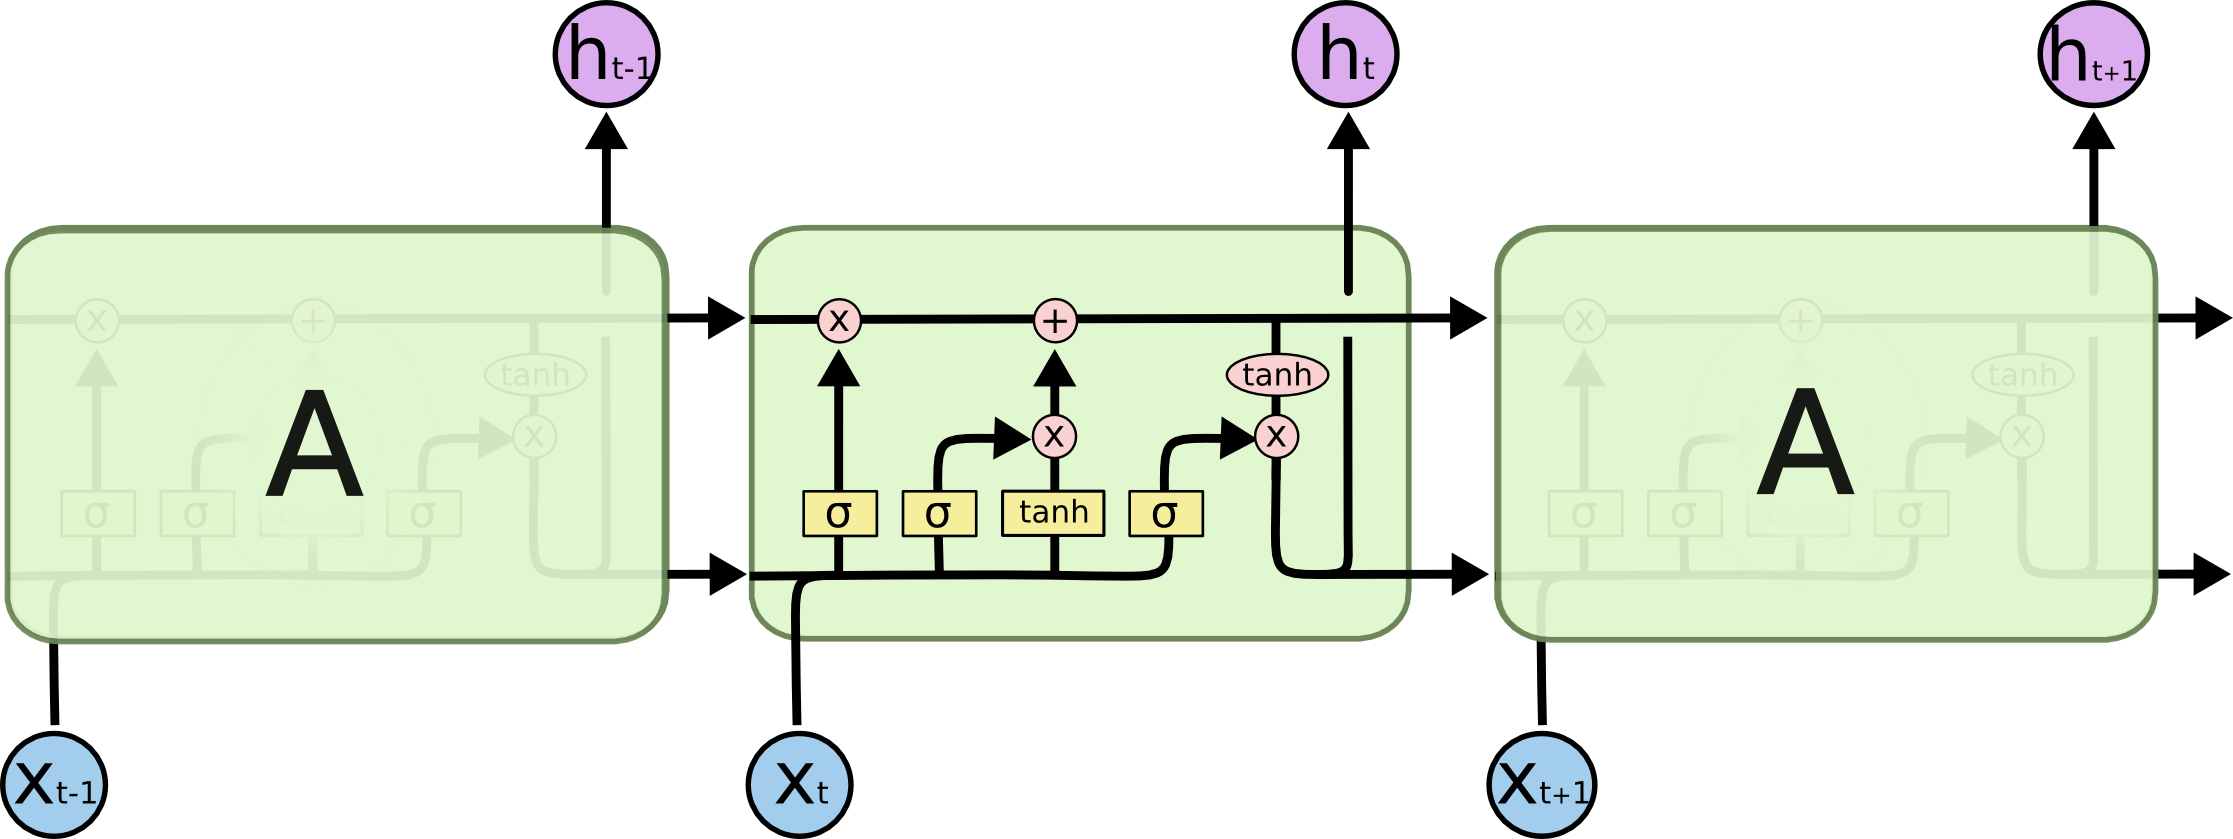
\includegraphics[scale=0.35]{pics/LSTMchain.png}
  \caption{Cadena desenrollada de una arquitectura LSTM.}
\end{figure}
\footnotetext{Fuente: \url{http://colah.github.io/posts/2015-08-Understanding-LSTMs/}}

Intuitivamente, las redes neuronales recurrentes pueden considerarse como redes de alimentación profunda con parámetros compartidos entre diferentes capas. En el caso de la RNN simple, los gradientes incluyen multiplicaciones repetidas de la matriz $W$, lo que hace que los valores de gradiente desaparezcan o exploten. El mecanismo de las compuertas mitiga este problema en gran medida al eliminar esta multiplicación repetida de una sola matriz. Las LSTMs son actualmente el tipo de arquitectura RNN más exitoso y son responsables de muchos resultados de modelado de secuencias de vanguardia. El principal competidor de la RNN LSTM es la GRU, que se discutirá a continuación.

\section{GRU}
La arquitectura LSTM es muy efectiva, pero también bastante complicada. La complejidad del sistema dificulta el análisis y también es computacionalmente costosa de trabajar. El Gated Recurrent Unit (GRU) se introdujo en \cite{cho2014learning} como una alternativa a LSTM. Posteriormente, se demostró en \cite{chung2014empirical} que tiene un rendimiento comparable a LSTM en varios conjuntos de datos (no textuales). Al igual que LSTM, GRU también se basa en un mecanismo de compuerta, pero con sustancialmente menos compuertas y sin un componente de memoria separado.

\begin{figure}[h]
  \centering
  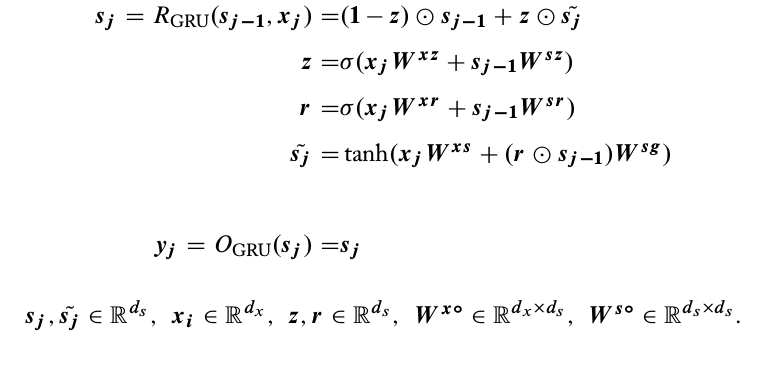
\includegraphics[scale=0.35]{pics/GRU.png}
  \caption{Arquitectura GRU.}
\end{figure}

Se utiliza una sola compuerta $\vec{r}$ para controlar el acceso al estado anterior $\vec{s}_{j-1}$ y calcular una actualización propuesta $\vec{\widetilde{s}}_j$. El estado actualizado $\vec{s}_j$ (que también sirve como salida $\vec{y}_j$) se determina luego en función de una interpolación entre el estado anterior $\vec{s}_{j-1}$ y la propuesta $\vec{\widetilde{s}}_j$. Las proporciones de la interpolación se controlan mediante la compuerta $\vec{z}$. Se ha demostrado que GRU es efectivo en el modelado del lenguaje y la traducción automática. Sin embargo, aún se está investigando y comparando la GRU, la LSTM y posibles arquitecturas de RNN alternativas. Para una exploración empírica de las arquitecturas GRU y LSTM, consulte \cite{jozefowicz2015empirical}.

\section{Clasificación de sentimientos con RNN}
El uso más simple de las RNN es como aceptores: leer una secuencia de entrada y producir una respuesta binaria o multi-clase al final. Las RNN son aprendices de secuencia muy poderosos y pueden captar patrones muy intrincados en los datos. Un ejemplo de oraciones naturalmente positivas y negativas en el dominio de las críticas de películas sería el siguiente: Positiva: "No es afirmativa de la vida, es vulgar y cruel, pero me gustó". Negativa: "Es decepcionante que solo logre ser decente en lugar de brillante".

Observa que el ejemplo positivo contiene algunas frases negativas ("no afirmativa de la vida", "vulgar" y "cruel"). Mientras que el ejemplo negativo contiene algunas frases positivas ("brillante"). Predecir correctamente el sentimiento requiere entender no solo las frases individuales sino también el contexto en el que ocurren, construcciones lingüísticas como la negación y la estructura general de la oración. La tarea de clasificación de sentimientos a nivel de oración se modela utilizando un RNN-aceptor. Después de la tokenización, la RNN lee las palabras de la oración una a la vez. Luego, el estado final de la RNN se alimenta a una MLP seguida de una capa softmax con dos salidas (positiva y negativa). La red se entrena con pérdida de entropía cruzada basada en las etiquetas de sentimiento correctas.

\begin{equation}
\begin{split}
p(\text{etiqueta}=k | \vec{w}_{1:n}) & = \hat{\vec{y}}_{[k]} \\
\hat{\vec{y}} & = \text{softmax}(\text{MLP}(\text{RNN}(\vec{x}_{1:n}))) \\
\vec{x}_{1:n} & = E_{[w_{1}]}, \dots, E_{[w_{n}]}
\end{split}
\end{equation}

La matriz de incrustación de palabras $E$ se inicializa utilizando incrustaciones pre-entrenadas aprendidas sobre un corpus externo grande utilizando un algoritmo como Word2vec o GloVe con una ventana relativamente amplia. A menudo es útil extender el modelo considerando RNN bidireccionales. Para oraciones más largas, \cite{li2015tree} encontró útil utilizar una arquitectura jerárquica, en la cual la oración se divide en segmentos más pequeños basados en la puntuación. Luego, cada segmento se alimenta a una RNN bidireccional. La secuencia de vectores resultantes (uno para cada segmento) se alimenta luego a un RNN aceptor. Se utilizó una arquitectura jerárquica similar para la clasificación de sentimientos a nivel de documento en \cite{tang2015document}.

\section{Clasificación de sentimientos en Twitter con LSTMS y Emojis}
Se propuso un modelo de supervisión remota basado en emojis para detectar sentimientos y otros estados afectivos en mensajes cortos de redes sociales en \cite{FelboMSRL17}. Se utilizan emojis como enfoque de supervisión remota para diversas tareas de detección afectiva (por ejemplo, emoción, sentimiento, sarcasmo) utilizando un corpus grande de 634 millones de tweets con 64 emojis. Se pre-entrena una arquitectura de red neuronal con este corpus. La red es una variante de LSTM formada por una capa de incrustación, 2 capas LSTM bidireccionales con conexiones de omisión normales y conexiones de agrupamiento promedio temporal.

\begin{figure}[h]
  \centering
  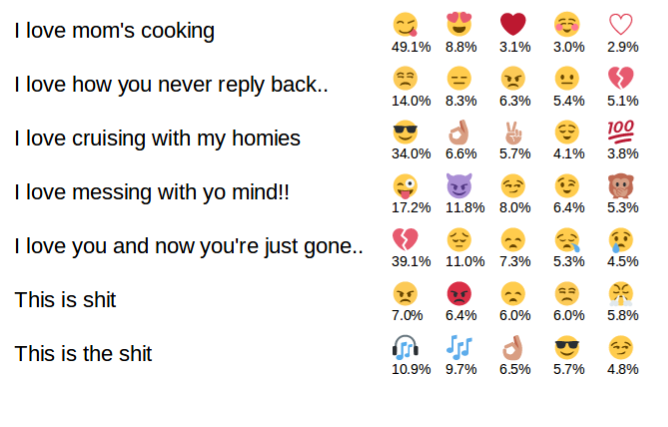
\includegraphics[scale=0.45]{pics/deepEmoji1.png}
  \caption{Arquitectura de red neuronal para la clasificación de sentimientos en Twitter con LSTMS y emojis (parte 1).}
\end{figure}

\begin{figure}[h]
  \centering
  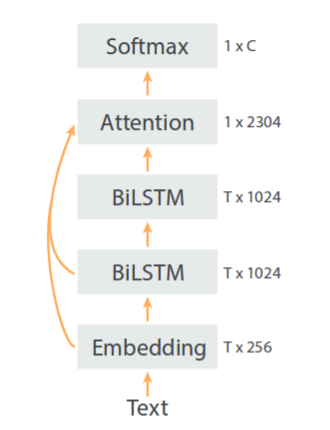
\includegraphics[scale=0.45]{pics/deepEmoji2.png}
  \caption{Arquitectura de red neuronal para la clasificación de sentimientos en Twitter con LSTMS y emojis (parte 2).}
\end{figure}

Los autores proponen el enfoque de transferencia de deshielo encadenado, en el cual la red pre-entrenada se ajusta finamente para la tarea objetivo. Aquí, cada capa se ajusta finamente individualmente en cada paso con los datos objetivos correctos, y luego todas se ajustan finamente juntas. El modelo logra resultados de vanguardia en la detección de emociones, sentimientos y sarcasmo. La red pre-entrenada se ha publicado para el público en

\begin{figure}[h]
  \centering
  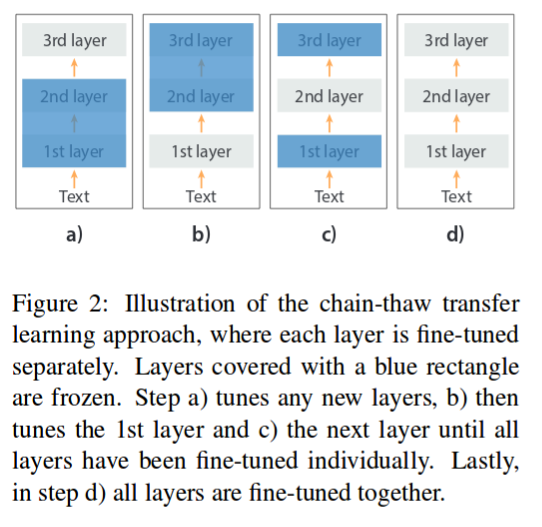
\includegraphics[scale=0.45]{pics/deepEmoji3.png}
  \caption{Demostración del modelo: \url{https://deepmoji.mit.edu/}.}
\end{figure}

\section{Bi-LSTM CRF}
Un enfoque alternativo al transductor para el etiquetado de secuencias es combinar una BI-LSTM con un Campo Aleatorio Condicional (CRF). Esto produce un etiquetador poderoso \cite{huang2015bidirectional} llamado BI-LSTM-CRF, en el cual la LSTM actúa como extractor de características y el CRF como una capa especial que modela las transiciones de una etiqueta a otra.

La capa CRF realiza una normalización global sobre todas las posibles secuencias, lo que ayuda a encontrar la secuencia óptima. En un CRF, modelamos la probabilidad condicional de la secuencia de etiquetas de salida dada la secuencia de entrada:

\begin{displaymath}
P(s_1, \dots, s_m | x_1, \dots, x_m) = P(s_{1:m}|x_{1:m})
\end{displaymath}

Lo hacemos definiendo un mapa de características $\vec{\Phi}(x_{1:m},s_{1:m}) \in \mathcal{R}^d$ que mapea una secuencia de entrada completa $x_{1:m}$ junto con una secuencia de etiquetas completa $s_{1:m}$ a un vector de características de $d$ dimensiones.

Luego, podemos modelar la probabilidad como un modelo log-lineal con el vector de parámetros $\vec{w} \in \mathcal{R}^d$:

\begin{displaymath}
P(s_{1:m}|x_{1:m}; \vec{w}) = \frac{\exp (\vec{w} \cdot \vec{\Phi}(x_{1:m},s_{1:m}))}{\sum_{s'_{1:m} \in S^m}\exp (\vec{w} \cdot \vec{\Phi}(x_{1:m},s'_{1:m}))}
\end{displaymath}

donde $s'_{1:m}$ varía sobre todas las posibles secuencias de salida.

Podemos ver la expresión $\vec{w} \cdot \vec{\Phi}(x_{1:m},s_{1:m})= \text{score}_{crf}(x_{1:m},s_{1:m})$ como una puntuación de qué tan bien se ajusta la secuencia de etiquetas a la secuencia de entrada dada.

Recordemos de la clase de CRF que $\vec{\Phi}(x_{1:m},s_{1:m})$ se creó con características diseñadas manualmente.

La idea del LSTM CRF es reemplazar $\vec{\Phi}(x_{1:m},s_{1:m})$ con la salida de un transductor LSTM (características aprendidas automáticamente):

\begin{displaymath}
\text{score}_{lstm-crf}(x_{1:m},s_{1:m})= \sum_{i=0}^{m} W_{[s_{i-1},s_i}]\cdot\text{LSTM}^*(x_{1:m})_{[i]} +\vec{b}{[s_{i-1},s_i]}
\end{displaymath}

donde $W_{[s_{i-1},s_i]}$ corresponde a una puntuación de transición de la etiqueta $s_{i-1}$ a $s_i$, $\vec{b}{[s_{i-1},s_i]}$ es un término de sesgo para la transición y $\text{LSTM}^*(x_{1:m})_{[i]}$ proviene del estado oculto de la Bi-LSTM en el paso de tiempo $i$.

Todos estos parámetros se aprenden conjuntamente. Observa que la matriz de transición $W$ no depende de la posición. Se utiliza el algoritmo de avance-retroceso durante el entrenamiento y el algoritmo de Viterbi durante la decodificación. Para obtener más información, consulta \footnote{\url{https://pytorch.org/tutorials/beginner/nlp/advanced_tutorial.html}} y \footnote{\url{https://www.depends-on-the-definition.com/sequence-tagging-lstm-crf/}}.
